% Appendix sections (included from acl.tex after \appendix)

\section{Configuration screening}
\label{app:validation}

Before locking the primary $(\text{pool}, \text{dataset}, \text{prompt formatting})$ triple, we screened candidates on small samples ($n{=}5$--$10$, seed 42) for non-degenerate routing opportunity and successful prefill extraction (\S\ref{sec:setup:config}).
Table~\ref{tab:config-screen} summarizes pilot outcomes.
Qwen~2.5~1.5B/3B on GSM8K ($n{=}5$) yielded 100\% too-hard buckets (both models failed all items).
The same Qwen pool on ARC ($n{=}10$) yielded 0\% opportunity with 70\% easy---weak model already succeeds on most items.
Llama~3.2~1B/3B on ARC showed 50\% opportunity on $n{=}10$ and ${\sim}24\%$ on a ${\sim}50$-query pilot, motivating the locked configuration reported in the main text ($n{=}1{,}172$ test; 43.3\% opportunity).

% Appendix: configuration screening (pilot samples; not reported metrics)
\begin{table}[t]
  \centering
  \small
  \begin{tabular}{llrrl}
    \toprule
    \textbf{Pool} & \textbf{Dataset} & $n$ & Opp.\ \% & \textbf{Outcome} \\
    \midrule
    Qwen 1.5B / 3B & GSM8K test & 5 & 0\% & Excluded: 100\% too-hard \\
    Qwen 1.5B / 3B & ARC-Challenge & 10 & 0\% & Excluded: 70\% easy \\
    Llama 1B / 3B & ARC-Challenge & 10 & 50\% & Studiable (pilot) \\
    Llama 1B / 3B & ARC-Challenge & ${\sim}50$ & ${\sim}24$\% & Non-degenerate mix \\
    \textbf{Llama 1B / 3B} & \textbf{ARC-Challenge} & \textbf{1{,}172} & \textbf{43.3\%} & \textbf{Locked (TEST)} \\
    \bottomrule
  \end{tabular}
  \caption{Requirements-first configuration search (seed 42). Pilot runs select a studiable $(\text{pool}, \text{dataset})$ triple; only the locked row contributes paper metrics.}
  \label{tab:config-screen}
\end{table}


\section{Complexity dimension candidate screening}
\label{app:d46}

Representative $c(q)$ is selected once on CALIB before test evaluation (\S\ref{sec:setup:calib}).
Table~\ref{tab:d46} reports all five tokenizer-based candidates scored against $y^{\text{opp}}$ on ARC validation ($n{=}299$).
\texttt{piece\_count} wins by the frozen composite rule despite modest absolute $\rho$ and AUROC; compressibility and normalized Shannon entropy rank higher on $|\rho|$ alone but lower on AUROC.
We report partial correlation $\rho(c,y^{\text{opp}}\mid\text{length})=-0.448$ on CALIB as a length-confound diagnostic for the selected feature.

% Appendix: D46 model-independent candidate screening (ARC CALIB, n=299)
\begin{table}[t]
  \centering
  \small
  \begin{tabular}{llccc}
    \toprule
    \textbf{Family} & \textbf{Candidate} & $\rho_s$ [95\% CI] & AUROC [95\% CI] & Composite \\
    \midrule
    Length & \texttt{piece\_count} & $+0.093$ [$-0.024$, $+0.210$] & $0.556$ [$0.486$, $0.629$] & 4.0 \\
    Lexical diversity & \texttt{mattr} & $-0.067$ [$-0.179$, $+0.048$] & $0.460$ [$0.395$, $0.530$] & 2.5 \\
    Information & \texttt{text\_shannon} & $-0.015$ [$-0.121$, $+0.099$] & $0.491$ [$0.426$, $0.560$] & 2.5 \\
    Information & \texttt{text\_shannon\_norm} & $-0.151$ [$-0.264$, $-0.039$] & $0.409$ [$0.345$, $0.481$] & 3.0 \\
    Compressibility & \texttt{compression\_ratio} & $-0.172$ [$-0.282$, $-0.061$] & $0.397$ [$0.328$, $0.465$] & 3.0 \\
    \bottomrule
  \end{tabular}
  \caption{D46 screening on ARC validation (CALIB, $n{=}299$). Selection maximizes composite $\tfrac{1}{2}\mathrm{rank}(|\rho|)+\tfrac{1}{2}\mathrm{rank}(\mathrm{AUROC})$; winner \texttt{piece\_count} frozen as $c(q)$ for all test reporting. Partial $\rho(c,y^{\text{opp}}\mid\text{length})=-0.448$ on CALIB (length confound diagnostic).}
  \label{tab:d46}
\end{table}


\section{Model-dependent probe variants}
\label{app:md-variants}

Prefill extraction logs auxiliary statistics from the same forward pass (\S\ref{sec:method:prefill}).
Table~\ref{tab:md-variants} audits redundancy on ARC test.
Normalized entropy, top-10 entropy, and effective vocabulary size $n_{\mathrm{eff}}=\exp(H_w)$ are numerically redundant with full-vocabulary $H_w$ ($\rho_s{\approx}1.0$; AUROC within 0.001).
Among derived cross-model statistics, $\Delta n_{\mathrm{eff}}$ achieves the highest opportunity AUROC (0.616) but does not change the recoverability interpretation relative to $\Delta m_{\mathrm{gain}}$ and $\Delta H$.

% Appendix: model-dependent probe variant redundancy (ARC TEST, n=1172)
\begin{table}[t]
  \centering
  \small
  \begin{tabular}{lccr}
    \toprule
    \textbf{Signal} & $\rho_s(H_w,\cdot)$ & Opp.\ AUROC & \textbf{Note} \\
    \midrule
    \multicolumn{4}{l}{\textit{Weak prefill variants}} \\
    $H_w$ (full vocab) & 1.000 & 0.581 & headline \\
    $H_{\mathrm{norm}}$ & 1.000 & 0.581 & redundant \\
    $H_{\mathrm{top10}}$ & 0.9998 & 0.580 & redundant \\
    $n_{\mathrm{eff}}$ & 1.000 & 0.581 & redundant ($e^{H_w}$) \\
    $m_w$ & $-0.819$ & 0.568$^\dagger$ & direction flipped \\
    $p_{\max}$ & $-0.911$ & 0.574$^\dagger$ & correlated with $H_w$ \\
  \addlinespace
    \multicolumn{4}{l}{\textit{Cross-model derived}} \\
    $\Delta H$ & --- & 0.602 & headline \\
    $\Delta H_{\mathrm{norm}}$ & --- & 0.601 & redundant \\
    $\Delta H_{\mathrm{top10}}$ & --- & 0.601 & redundant \\
    $\Delta n_{\mathrm{eff}}$ & --- & 0.616 & best single AUROC \\
    $\Delta m_{\mathrm{gain}}$ & --- & 0.605 & recoverability rep. \\
    \bottomrule
  \end{tabular}
  \caption{Probe variant audit on ARC test. $^\dagger$AUROC after sign flip (higher score $\Rightarrow$ higher opportunity). Variants logged at extraction time; main text uses $H_w$, $m_w$, $\Delta H$, $\Delta m_{\mathrm{gain}}$ only.}
  \label{tab:md-variants}
\end{table}


\section{Information dimension taxonomy (extended)}
\label{app:dimensions}

Table~\ref{tab:dim-taxonomy} lists candidate statistics for each information dimension.
The main analysis reports bold representatives only; additional rows indicate future measurements without expanding headline claims.

% Extended dimension taxonomy (candidates; not main-paper claims). Bold rows match Table~\ref{tab:dimensions}.
\begin{table}[t]
  \centering
  \footnotesize
  \setlength{\tabcolsep}{3pt}
  \begin{tabular}{@{}p{0.14\linewidth}p{0.20\linewidth}p{0.58\linewidth}@{}}
    \toprule
    \textbf{Dimension} & \textbf{Source} & \textbf{Candidate statistics; main study in bold} \\
    \midrule
    \textbf{Complexity} & Query text &
    \textbf{\texttt{piece\_count}}, MATTR, MTLD, compression, text Shannon, sentence count, choice count, prompt length \\
    \addlinespace
    \textbf{Uncertainty} & $M_i$ logits &
    \textbf{$H$}, $H_{\mathrm{top10}}$, $n_{\mathrm{eff}}$, tail entropy, R\'enyi \\
    \addlinespace
    Confidence & $M_i$ logits &
    \textbf{$m$}, $p_{\max}$, top-5 mass, log-odds \\
    \addlinespace
    \textbf{Agreement} & $M_w{\leftrightarrow}M_s$ &
    \textbf{$\Delta H$}, KL, JS divergence, rank correlation \\
    \addlinespace
    \textbf{Recoverability} & $M_w{\leftrightarrow}M_s$ &
    \textbf{$\Delta m_{\mathrm{gain}}$}, $\Delta p_{\max}$, $\Delta n_{\mathrm{eff}}$ \\
    \addlinespace
    Dynamics & Generation trajectory &
    entropy slope, margin slope, trajectory variance (future work) \\
    \addlinespace
    Representation & Hidden states &
    layer norms, hidden similarity (future work) \\
    \addlinespace
    Stability & Paraphrase / multi-probe &
    cross-paraphrase variance (deferred) \\
    \addlinespace
    Calibration & Offline fit &
    ECE, temperature, Brier (deferred) \\
    \bottomrule
  \end{tabular}
  \caption{Extended information-dimension taxonomy. Main text reports bold representatives only; additional rows indicate future measurements without expanding headline claims.}
  \label{tab:dim-taxonomy}
\end{table}


\section{Calibration diagnostics}
\label{app:calibration}

Figure~\ref{fig:entropy-calib} shows weak entropy $H_w$ quantile calibration against opportunity rate on TEST (decile bins).
Figure~\ref{fig:prob-calib} shows probability calibration of the joint logistic model from Study~IV (CALIB-fit, TEST-eval).
The joint model is underconfident (mean signed gap $-0.037$ per bin), consistent with degenerate routing $\tau{=}0$ on TEST (\S\ref{sec:routing:results}).

\begin{figure}[t]
  \centering
  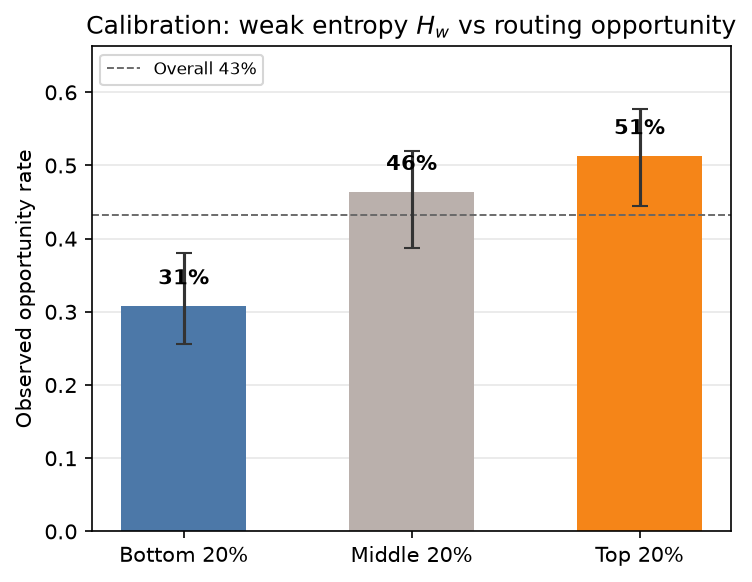
\includegraphics[width=0.92\linewidth]{figures/F4_entropy_calibration.png}
  \caption{Weak entropy $H_w$ quantile calibration vs.\ observed opportunity rate (ARC test).}
  \label{fig:entropy-calib}
\end{figure}

\begin{figure}[t]
  \centering
  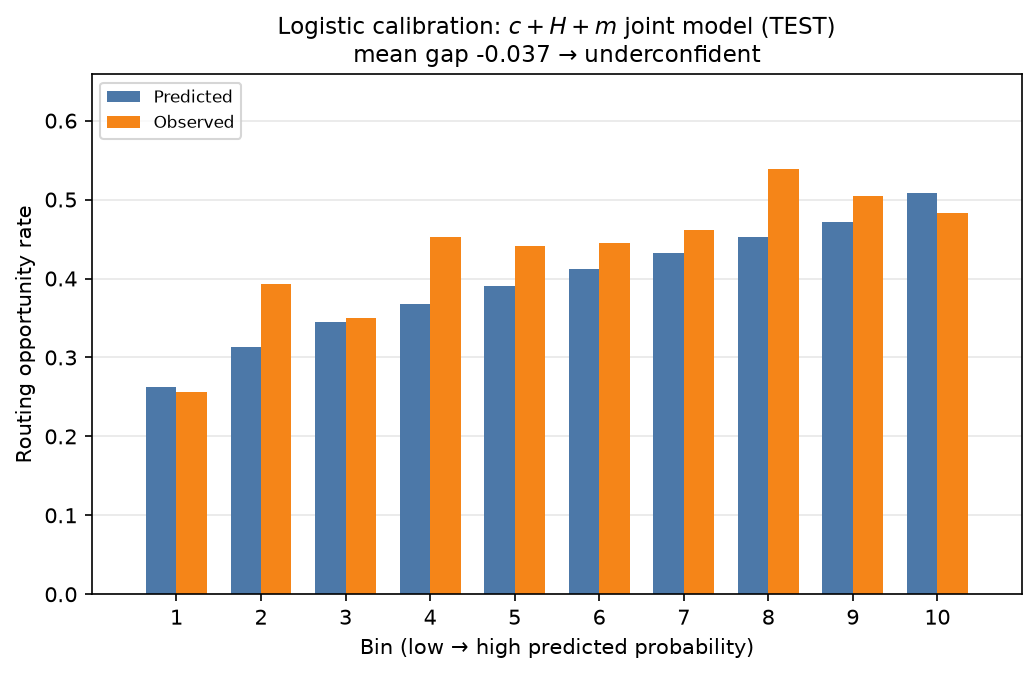
\includegraphics[width=0.92\linewidth]{figures/F5_probability_calibration.png}
  \caption{Joint logistic $\Pr(y^{\text{opp}}\mid c,H_w,m_w)$ calibration (CALIB-fit, TEST-eval).}
  \label{fig:prob-calib}
\end{figure}
